\section{تولید قواعد وابستگی}

% Slide 23
\begin{frame}{از مجموعه‌آیتم‌های مکرر به قواعد}{\lr{From Frequent Itemsets to Rules}}
\begin{columns}[T,onlytextwidth]
\begin{column}{0.56\textwidth}
\begin{itemize}\setlength{\itemsep}{4pt}\small
    \item \textbf{مسئله:} به‌ازای مجموعه‌آیتم مکرر داده‌شده $L$، تمام زیرمجموعه‌های ناتهی $f \subset L$ را بیابید به‌گونه‌ای که قاعدهٔ زیر شرط حداقل اطمینان (\lr{minconf}) را برآورده سازد:
    \par\vspace{1pt}\noindent\makebox[\linewidth][c]{$f \to L \setminus f$}\par\vspace{2pt}
    \item \textbf{مثال مجموعه‌آیتم مکرر}: فرض کنید $L = \{\text{\lr{Milk, Diaper, Beer}}\}$
    \item \textbf{مثال قاعدهٔ وابستگی}:
    \par\vspace{1pt}\noindent\makebox[\linewidth][c]{$\underbrace{\{\text{\lr{Milk, Diaper}}\}}_f \to \{\text{\lr{Beer}}\}$}\par\vspace{2pt}
    \par\vspace{1pt}\noindent\makebox[\linewidth][c]{$\displaystyle c = \frac{\sigma(\text{\lr{Milk, Diaper, Beer}})}{\sigma(\text{\lr{Milk, Diaper}})} = \frac{2}{3} \approx 0.67$}\par\vspace{2pt}
\end{itemize}
\end{column}%
\begin{column}{0.40\textwidth}
\centering
\textbf{\small تراکنش‌های خرید}\\[1pt]
{\scriptsize\lr{(Shopping Transactions)}}\\[3pt]
\begin{latin}
\fontsize{7.5}{9.5}\selectfont
\begin{tabular}{|c|l|}
\hline
\rowcolor{mannheimblue!15}
\textbf{TID} & \textbf{Items} \\ \hline
1 & Bread, Milk \\ \hline
2 & Bread, Diaper, Beer, Eggs \\ \hline
3 & Milk, Diaper, Beer, Coke \\ \hline
4 & Bread, Milk, Diaper, Beer \\ \hline
5 & Bread, Milk, Diaper, Coke \\ \hline
\end{tabular}
\end{latin}
\end{column}
\end{columns}
\end{frame}

% Slide 24
\begin{frame}{چالش: انفجار ترکیبیاتی}{\lr{Challenge: Combinatorial Explosion}}
\begin{itemize}\setlength{\itemsep}{4pt}
    \item برای یک مجموعه‌آیتم ۴عضوی $\{A, B, C, D\}$، می‌توان قواعد زیر را تولید کرد:
    \begin{center}
    \small
    \renewcommand{\arraystretch}{1.2}
    \begin{tabular}{lll}
    $\{A\} \to \{B,C,D\}$ & $\{A,B\} \to \{C,D\}$ & $\{A,B,C\} \to \{D\}$ \\
    $\{B\} \to \{A,C,D\}$ & $\{A,C\} \to \{B,D\}$ & $\{A,B,D\} \to \{C\}$ \\
    $\{C\} \to \{A,B,D\}$ & $\{A,D\} \to \{B,C\}$ & $\{A,C,D\} \to \{B\}$ \\
    $\{D\} \to \{A,B,C\}$ & $\{B,C\} \to \{A,D\}$ & $\{B,C,D\} \to \{A\}$ \\
    & $\{B,D\} \to \{A,C\}$ & \\
    & $\{C,D\} \to \{A,B\}$ & \\
    \end{tabular}
    \end{center}
    \item یعنی در مجموع \textbf{۱۴ قاعده} تنها از یک مجموعه‌آیتم ۴عضوی!
    \item \textbf{فرمول کلی تعداد قواعد برای یک مجموعه‌آیتم $k$‌عضوی:}
    \[
    2^k - 2
    \]
    \begin{itemize}\footnotesize
        \item برابر $2^k$ نیست زیرا قواعد بدیهی $\emptyset \to \{\dots\}$ و $\{\dots\} \to \emptyset$ نادیده گرفته می‌شوند.
    \end{itemize}
\end{itemize}
\end{frame}

% Slide 25
\begin{frame}{چالش: انفجار ترکیبیاتی}{\lr{Challenge: Combinatorial Explosion}}
\begin{columns}[T,onlytextwidth]
\begin{column}{0.56\textwidth}
\begin{itemize}\setlength{\itemsep}{4pt}\small
    \item \textbf{هدف مطلوب:} یافتن یک ترفند هرس دیگر مشابه اصل آپریوری.
    \item \textbf{با این حال، به مثال‌های زیر دقت کنید:}
    \begin{itemize}\footnotesize
        \item $c(\{\text{Milk}, \text{Diaper}\} \to \{\text{Beer}\}) = 0.67$
        \item $c(\{\text{Milk}\} \to \{\text{Beer}\}) = 0.5$
        \item $c(\{\text{Diaper}\} \to \{\text{Beer}\}) = 0.8$
        \item مقدار $c(ABC \to D)$ می‌تواند بزرگ‌تر یا کوچک‌تر از $c(AB \to D)$ باشد!
    \end{itemize}
    \vspace{0.2cm}
    \item \alert{\textbf{نتیجه‌گیری:}} به‌طور کلی، معیار اطمینان (\lr{confidence}) دارای \textbf{خاصیت پاد‌یکنواختی نیست}!
\end{itemize}
\end{column}%
\begin{column}{0.40\textwidth}
\centering
\textbf{\small تراکنش‌های خرید}\\[1pt]
{\scriptsize\lr{(Shopping Transactions)}}\\[3pt]
\begin{latin}
\fontsize{7.5}{9.5}\selectfont
\begin{tabular}{|c|l|}
\hline
\rowcolor{mannheimblue!15}
\textbf{TID} & \textbf{Items} \\ \hline
1 & Bread, Milk \\ \hline
2 & Bread, Diaper, Beer, Eggs \\ \hline
3 & Milk, Diaper, Beer, Coke \\ \hline
4 & Bread, Milk, Diaper, Beer \\ \hline
5 & Bread, Milk, Diaper, Coke \\ \hline
\end{tabular}
\end{latin}
\end{column}
\end{columns}
\end{frame}

% Slide 26
\begin{frame}{چالش: انفجار ترکیبیاتی}{\lr{Challenge: Combinatorial Explosion}}
\begin{columns}[T,onlytextwidth]
\begin{column}{0.63\textwidth}
\begin{itemize}\setlength{\itemsep}{2pt}\footnotesize
    \item \textbf{اما:} اطمینان قواعدی که \textbf{از یک مجموعه‌آیتم یکسان} مشتق می‌شوند، دارای خاصیت پاد‌یکنواختی است.
    \item برای مثال، فرض کنید مجموعه‌آیتم $L = \{\text{Milk}, \text{Diaper}, \text{Beer}\}$ باشد:
    \begin{itemize}\setlength{\itemsep}{1pt}\scriptsize
        \item $\{\text{Milk}, \text{Diaper}, \text{Beer}\} \to \emptyset \quad (c = 1.0)$
        \item $\{\text{Milk}, \text{Diaper}\} \to \{\text{Beer}\} \quad (c = 0.67)$
        \item $\{\text{Milk}, \text{Beer}\} \to \{\text{Diaper}\} \quad (c = 1.0)$
        \item $\{\text{Beer}\} \to \{\text{Milk}, \text{Diaper}\} \quad (c = 0.67)$
        \item $\{\text{Milk}\} \to \{\text{Diaper}, \text{Beer}\} \quad (c = 0.5)$
        \item $\{\text{Diaper}\} \to \{\text{Milk}, \text{Beer}\} \quad (c = 0.5)$
    \end{itemize}
    \item برای مجموعه‌آیتم $L = \{A, B, C, D\}$ داریم:
    \par\vspace{1pt}\noindent\makebox[\linewidth][c]{$\displaystyle c(ABC \to D) \ge c(AB \to CD) \ge c(A \to BCD)$}\par\vspace{1pt}
\end{itemize}

\vspace{-0.1cm}
\begin{tcolorbox}[colback=mannheimgold!15,colframe=mannheimgold!80!black,arc=2pt,left=3pt,right=3pt,top=2pt,bottom=2pt]
\scriptsize \textbf{مشاهده:} انتقال مؤلفه‌ها از مقدم به مؤخر («از چپ به راست») در یک قاعده، \textbf{هرگز اطمینان را افزایش نمی‌دهد}!
\end{tcolorbox}
\end{column}%
\begin{column}{0.35\textwidth}
\centering
\textbf{\small تراکنش‌های خرید}\\[1pt]
{\scriptsize\lr{(Shopping Transactions)}}\\[3pt]
\begin{latin}
\fontsize{7.5}{9.5}\selectfont
\begin{tabular}{|c|l|}
\hline
\rowcolor{mannheimblue!15}
\textbf{TID} & \textbf{Items} \\ \hline
1 & Bread, Milk \\ \hline
2 & Bread, Diaper, Beer, Eggs \\ \hline
3 & Milk, Diaper, Beer, Coke \\ \hline
4 & Bread, Milk, Diaper, Beer \\ \hline
5 & Bread, Milk, Diaper, Coke \\ \hline
\end{tabular}
\end{latin}
\end{column}
\end{columns}
\end{frame}

% Slide 27
\begin{frame}{توضیح ریاضی پاد‌یکنواختی اطمینان}{\lr{Explanation}}
\begin{itemize}\setlength{\itemsep}{5pt}
    \item اطمینان نسبت به \textbf{تعداد آیتم‌های سمت راست (\lr{RHS}) قاعده} پاد‌یکنوا است:
    \begin{itemize}\setlength{\itemsep}{2pt}
        \item به این معنی که: انتقال عناصر از چپ به راست نمی‌تواند اطمینان را افزایش دهد.
    \end{itemize}
    \item \textbf{علت ریاضی:}
    \begin{itemize}\setlength{\itemsep}{2pt}
        \item به دلیل ویژگی پاد‌یکنواختی پشتیبان، می‌دانیم که $s(AB) \le s(A)$ است.
        \item با توجه به تعریف اطمینان:
        \begin{latin}
        \[
        c(AB \to C) \coloneqq \frac{s(ABC)}{s(AB)}, \qquad c(A \to BC) \coloneqq \frac{s(ABC)}{s(A)}
        \]
        \end{latin}
        \item چون صورت هر دو کسر یکسان است و مخرج کسر اول کوچک‌تر یا مساوی است یعنی $s(AB) \le s(A)$، در نتیجه:
        \[
        c(AB \to C) \ge c(A \to BC)
        \]
    \end{itemize}
\end{itemize}
\end{frame}

% Slide 28
\begin{frame}{هرس قواعد نامزد}{\lr{Candidate Rule Pruning}}
\begin{itemize}\setlength{\itemsep}{3pt}
    \item \textbf{انتقال عناصر از چپ به راست نمی‌تواند اطمینان را افزایش دهد:}
    \begin{itemize}
        \item اگر یک قاعده دارای اطمینان پایینی باشد، تمامی قواعد مشتق‌شده از آن با انتقال آیتم به سمت راست نیز اطمینان پایینی خواهند داشت و بلافاصله هرس می‌شوند.
    \end{itemize}
\end{itemize}

\vspace{-0.1cm}
\begin{center}
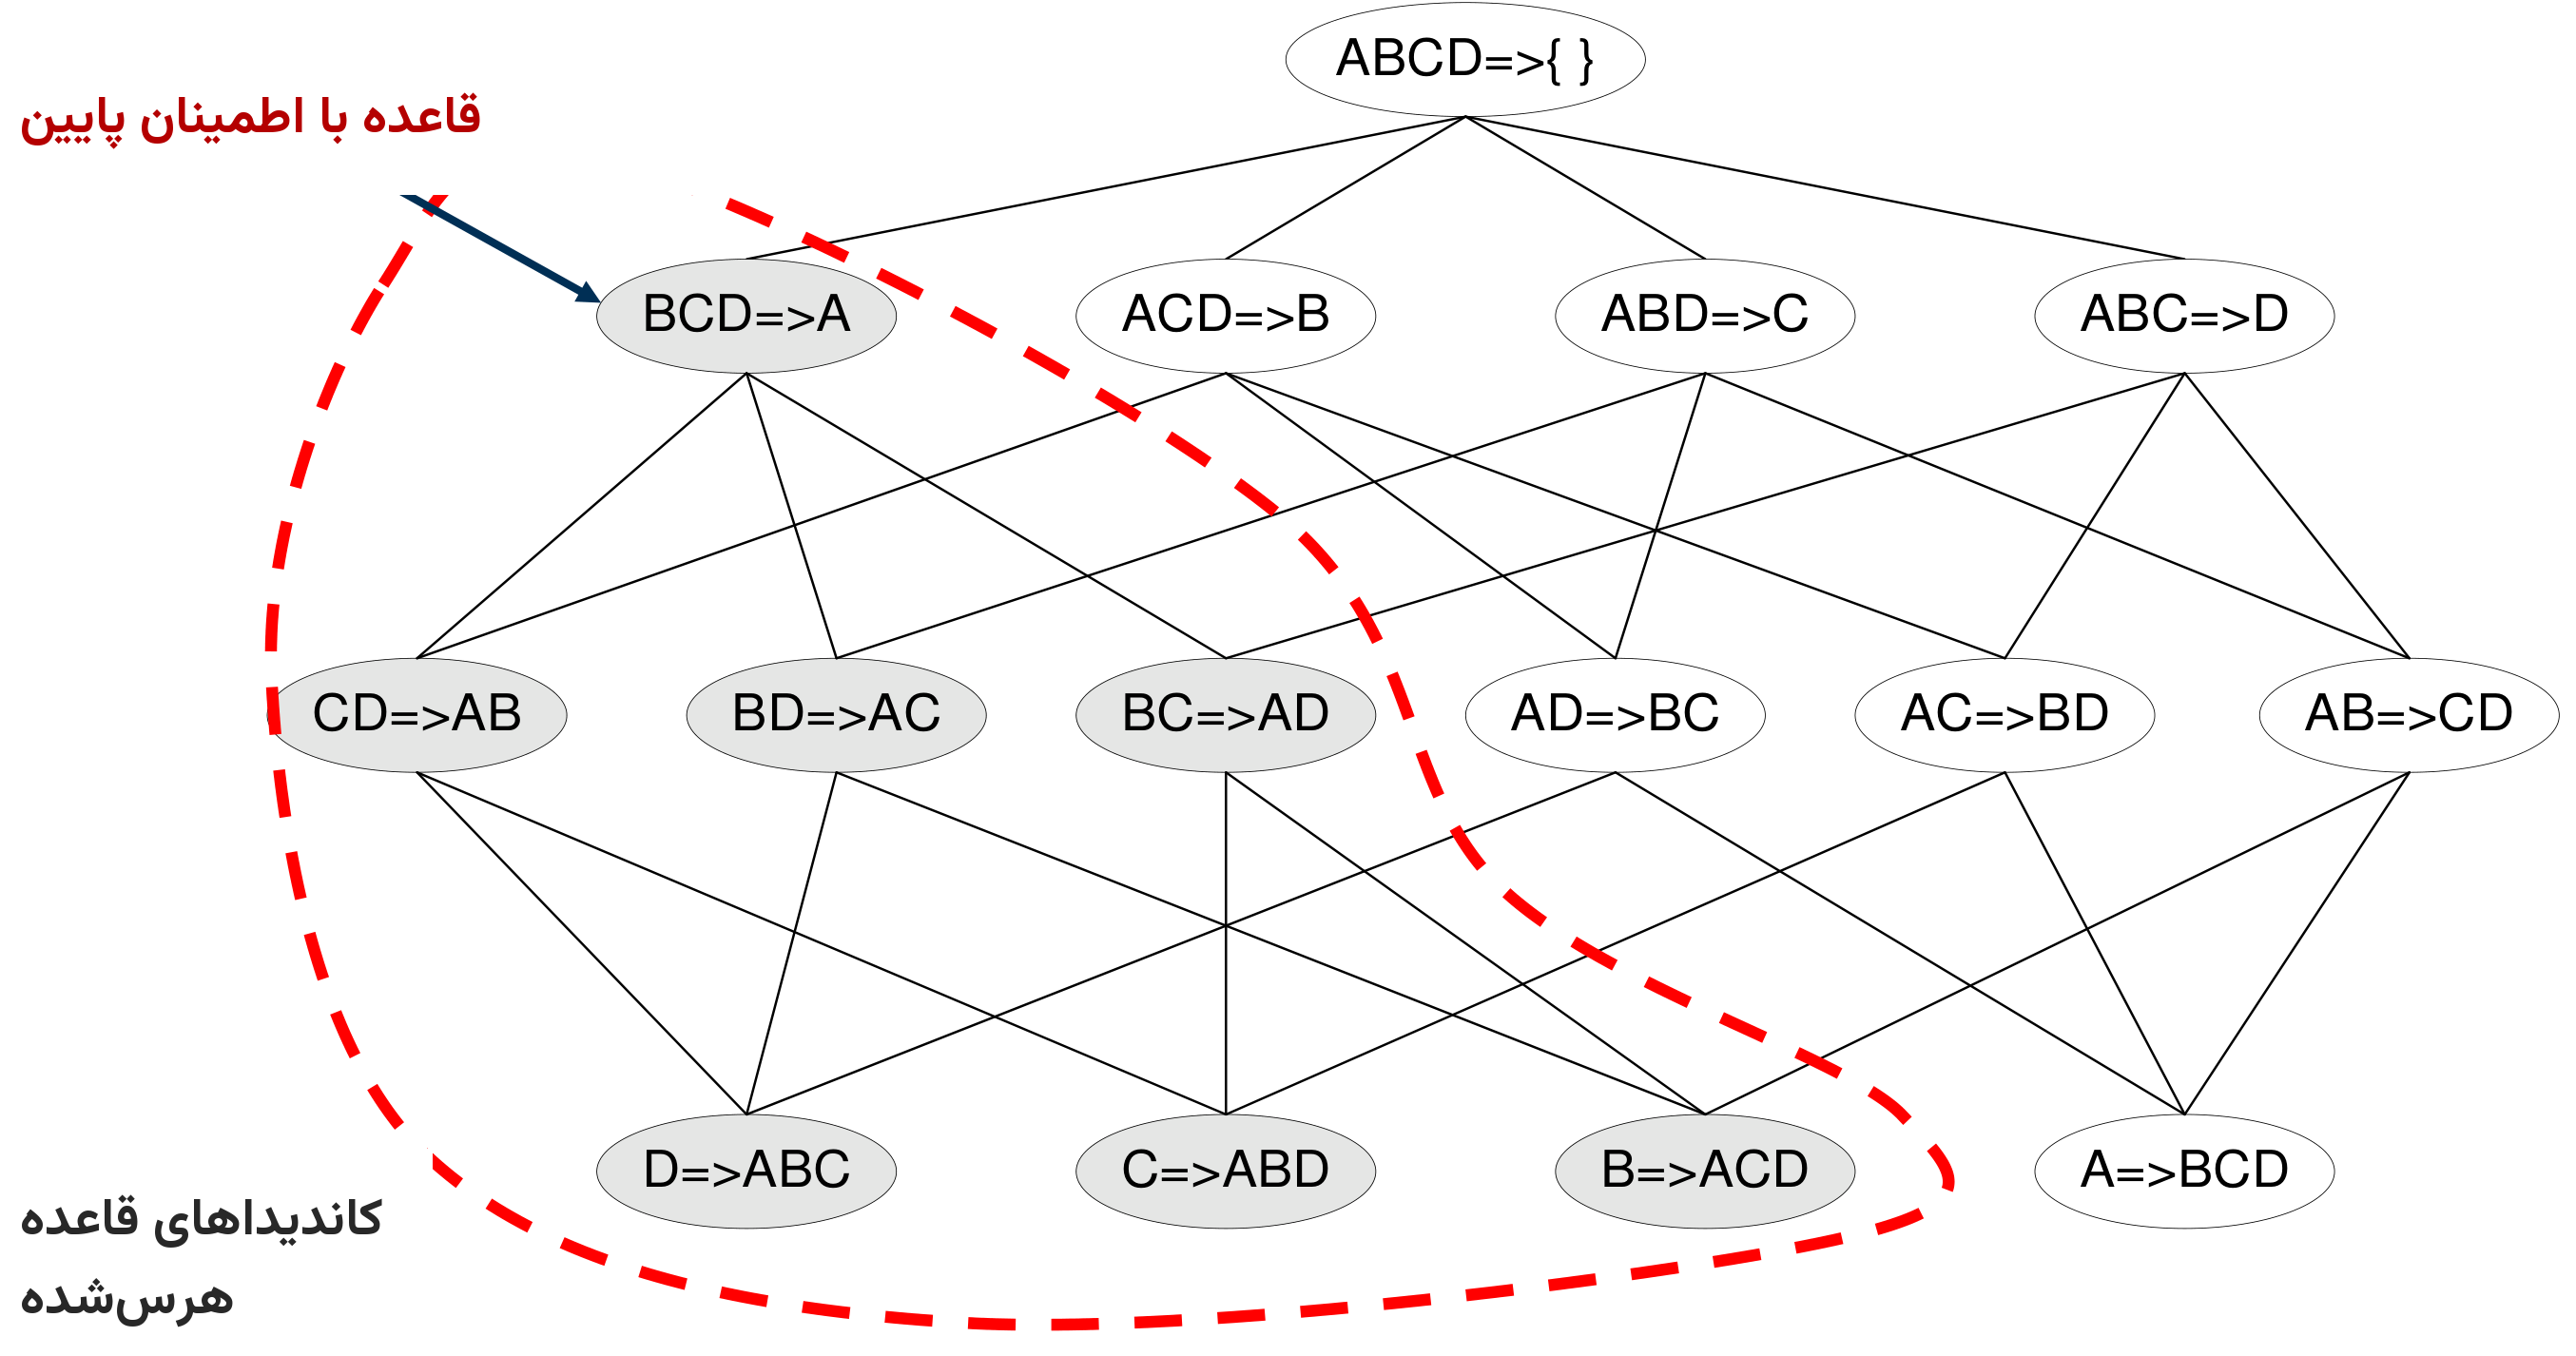
\includegraphics[width=0.76\textwidth,keepaspectratio]{images/slide28_lattice_fa.png}
\end{center}
\end{frame}

% Slide 29
\begin{frame}{تولید قاعده برای الگوریتم آپریوری}{\lr{Rule Generation for Apriori Algorithm}}
\begin{columns}[T,onlytextwidth]
\begin{column}{0.68\textwidth}
\begin{itemize}\setlength{\itemsep}{4pt}\small
    \item \textbf{قاعدهٔ کاندید} با ادغام دو قاعده‌ای تولید می‌شود که دارای پیشوند یکسانی در مؤخر (\lr{consequent}) قاعده باشند:
    \begin{itemize}\footnotesize
        \item ادغام $\mathrm{join}(CD \to AB,\, BD \to AC)$ قاعدهٔ کاندید $D \to ABC$ را تولید می‌کند.
        \item اگر یکی از قواعد والد (مانند $AD \to BC$) اطمینان بالایی نداشته باشد، قاعدهٔ $D \to ABC$ \textbf{هرس} می‌شود.
    \end{itemize}
\end{itemize}
\end{column}%
\begin{column}{0.30\textwidth}
\centering
\vspace{0.1cm}
\begin{tikzpicture}[box/.style={draw=mannheimblue, fill=blue!5, rounded corners=3pt, font=\small\bfseries, inner sep=5pt}]
  \node[box] (cd) at (0, 1.4) {$CD \Rightarrow AB$};
  \node[box] (bd) at (2.2, 1.4) {$BD \Rightarrow AC$};
  \node[box, fill=orange!15, draw=orange!80!black] (d) at (1.1, 0) {$D \Rightarrow ABC$};
  \draw[->, thick, mannheimblue] (cd) -- (d);
  \draw[->, thick, mannheimblue] (bd) -- (d);
\end{tikzpicture}
\end{column}
\end{columns}

\vspace{0.25cm}
\begin{itemize}\setlength{\itemsep}{4pt}\small
    \item \textbf{نکته کلیدی:} تمام اطلاعات موردنیاز برای محاسبهٔ اطمینان قبلاً در مرحلهٔ تولید مجموعه‌آیتم‌ها ذخیره شده است:
    \par\vspace{2pt}\noindent\makebox[\linewidth][c]{$\displaystyle c(X \to Y) = \frac{s(X \cup Y)}{s(X)}$}\par\vspace{2pt}
    \begin{itemize}\footnotesize
        \item در نتیجه، \textbf{هیچ نیازی به پیمایش مجدد داده‌ها وجود ندارد!}
    \end{itemize}
\end{itemize}
\end{frame}
